\documentclass[hyperref=unicode,presentation,10pt]{beamer}

\usepackage[absolute,overlay]{textpos}
\usepackage{array}
\usepackage{graphicx}
\usepackage{adjustbox}
\usepackage[version=4]{mhchem}
\usepackage{chemfig}
\usepackage{caption}
\usepackage{makecell}

%dělení slov
\usepackage{ragged2e}
\let\raggedright=\RaggedRight
%konec dělení slov

\addtobeamertemplate{frametitle}{
	\let\insertframetitle\insertsectionhead}{}
\addtobeamertemplate{frametitle}{
	\let\insertframesubtitle\insertsubsectionhead}{}

\makeatletter
\CheckCommand*\beamer@checkframetitle{\@ifnextchar\bgroup\beamer@inlineframetitle{}}
\renewcommand*\beamer@checkframetitle{\global\let\beamer@frametitle\relax\@ifnextchar\bgroup\beamer@inlineframetitle{}}
\makeatother
\setbeamercolor{section in toc}{fg=red}
\setbeamertemplate{section in toc shaded}[default][100]

\usepackage{fontspec}
\usepackage{unicode-math}

\usepackage{polyglossia}
\setdefaultlanguage{czech}

\def\uv#1{„#1“}

\mode<presentation>{\usetheme{default}}
\usecolortheme{crane}

\setbeamertemplate{footline}[frame number]

\title[Crisis]
{C2062 -- Anorganická chemie II}

\subtitle{Osmium, iridium, platina, hassium, meitnerium a darmstadtium}
\author{Zdeněk Moravec, hugo@chemi.muni.cz \\ \adjincludegraphics[height=60mm]{img/IUPAC_PSP.jpg}}
\date{}

\begin{document}

\begin{frame}
	\titlepage
\end{frame}

\section{Úvod}
\frame{
	\frametitle{}
	\vfill
	\begin{tabular}{|c|l|l|l|}
	\hline
	 & \textit{Osmium} & \textit{Iridium} & \textit{Platina} \\\hline
	 El. konfigurace & 4f$^{10}$ 5d$^{6}$ 6s$^{2}$ & 4f$^{10}$ 5d$^{7}$ 6s$^{2}$ & 4f$^{10}$ 5d$^{9}$ 6s$^{1}$ \\\hline
	 Teplota tání [$^\circ$C] & 3033 & 2446 & 1768 \\\hline
	 Teplota varu [$^\circ$C]  & 5012 & 4130 & 3825 \\\hline
	 Objeven & 1803 & 1803 & 1735 \\\hline
	 Vzhled & stříbrný\footnote[frame]{Zdroj: \href{https://commons.wikimedia.org/wiki/File:Osmium_crystals.jpg}{Alchemist-hp/Commons}} & stříbrno-bílý\footnote[frame]{Zdroj: \href{https://commons.wikimedia.org/wiki/File:Iridium-2.jpg}{Materialscientist/Commons}} & stříbrno-bílý\footnote[frame]{Zdroj: \href{https://commons.wikimedia.org/wiki/File:Platinum_crystals.jpg}{Periodictableru/Commons}} \\
	 &  \begin{minipage}{.2\textwidth}
	 	\adjincludegraphics[width=\linewidth]{img/Osmium_crystals.jpg}
	 \end{minipage}
	 	& \begin{minipage}{.2\textwidth}
	 		\adjincludegraphics[width=\linewidth]{img/Iridium.jpg}
	 	\end{minipage} & \begin{minipage}{.2\textwidth}
	 	\adjincludegraphics[width=\linewidth]{img/Platina.jpg}
 	\end{minipage} \\\hline
	\end{tabular}
	\vfill
}
\section{Hassium, meitnerium a darmstadtium}
\subsection{Hassium}
\frame{
	\frametitle{}
	\begin{columns}
		\begin{column}{0.6\textwidth}
			\vfill
			\begin{itemize}
				\item \textit{Hassium}, transuran s protonovým číslem 108.
				\item Nemá žádný stabilní izotop.
				\item Pojmenován byl v roce 1997 podle spolkového státu Hesensko, kde byl poprvé připraven.\footnote[frame]{\href{http://publications.iupac.org/pac/pdf/1997/pdf/6912x2471.pdf}{Names and symbols of transfermium elements}}
				\item První příprava byla publikována roku 1984, kdy byl terč z olova bombardován jádry železa:
				\item \ce{$_{\ 82}^{208}$Pb + $_{26}^{58}$Fe -> $^{265}_{108}$Hs + ^1_0n}
				\item Známe 12 izotopů a tři jaderné izomery. Nejdelší poločas rozpadu má \ce{^{277m}Hs}, 110~s.
			\end{itemize}
			\vfill
		\end{column}
		\begin{column}{0.4\textwidth}
			\begin{figure}
				\adjincludegraphics[width=.9\textwidth]{img/Hesse.png}
				\caption*{Hesensko.\footnote[frame]{Zdroj: \href{https://commons.wikimedia.org/wiki/File:Locator_map_Hesse_in_Germany.svg}{TUBS/Commons}}}
			\end{figure}
		\end{column}
	\end{columns}
}

\frame{
	\frametitle{}
		\vfill
		\begin{itemize}
			\item U hassia se předpokládá vyšší stabilita oxidačního stavu VIII.
			\item Hassium lze oxidovat na \ce{HsO4} při teplotě 600~$^\circ$C.\footnote[frame]{\href{https://web.archive.org/web/20120311001032/http://www.gsi.de/documents/DOC-2003-Jun-29-2.pdf}{Chemistry of Hassium}}
			\item \ce{Hs + 2 O2 ->[He, 600 $^\circ$C] HsO4}
			\item Reakcí oxidu s alkalickými hydroxidy vznikají bazické hassičelany:
			\item \ce{HsO4 + 2 NaOH -> Na2[HsO4(OH)2]}
		\end{itemize}
		\vfill
}

\subsection{Meitnerium}
\frame{
	\frametitle{}
	\begin{columns}
		\begin{column}{0.6\textwidth}
			\vfill
			\begin{itemize}
				\item \textit{Meitnerium}, transuran s protonovým číslem 109.
				\item Nemá žádný stabilní izotop.
				\item Pojmenován byl v roce 1997 podle rakouské fyzičky Lise Meitner, která se zabývala studiem radioaktivity.\footnote[frame]{\href{http://publications.iupac.org/pac/pdf/1997/pdf/6912x2471.pdf}{Names and symbols of transfermium elements}}
				\item První příprava byla publikována roku 1982, terč z bismutu byl bombardován jádry železa:
				\item \ce{$_{\ 83}^{209}$Bi + $_{26}^{58}$Fe -> $^{266}_{109}$Mt + ^1_0n}
				\item Známe devět izotopů a dva jaderné izomery. Nejdelší poločas rozpadu má \ce{^{278}Mt}, 7,6~s.
			\end{itemize}
			\vfill
		\end{column}
		\begin{column}{0.4\textwidth}
			\begin{figure}
				\adjincludegraphics[width=\textwidth]{img/Hahn_Meitner_1912.jpg}
				\caption*{Lisa Mietnerová a Otto Hahn, 1912.\footnote[frame]{Zdroj: \href{https://commons.wikimedia.org/wiki/File:Hahn_Meitner_1912.jpg}{Drdoht/Commons}}}
			\end{figure}
		\end{column}
	\end{columns}
}

\subsection{Darmstadtium}
\frame{
	\frametitle{}
	\begin{columns}
		\begin{column}{0.6\textwidth}
			\vfill
			\begin{itemize}
				\item \textit{Darmstadtium}, transuran s protonovým číslem 110.
				\item Nemá žádný stabilní izotop.
				\item Pojmenován byl v roce 2003 podle německého Darmstadtu.\footnote[frame]{\href{https://doi.org/10.1351/pac200375101613}{Name and Symbol of the Element with Atomic Number 110 (IUPAC Recommendations 2003)}}
				\item První příprava byla publikována roku 1994, kdy byl terč z olova bombardován jádry niklu:\footnote[frame]{\href{https://doi.org/10.1007/BF01291181}{Production and decay of $^{269}$110}}
				\item \ce{$_{\ 82}^{208}$Pb + $_{28}^{62}$Ni -> $^{269}_{110}$Ds + ^1_0n}
				\item \ce{$_{\ 82}^{208}$Pb + $_{28}^{64}$Ni -> $^{271}_{110}$Ds + ^1_0n}
				\item Známe devět izotopů a tři jaderné izomery. Nejdelší poločas rozpadu má \ce{^{281}Ds}, 9,6~s.
			\end{itemize}
			\vfill
		\end{column}
		\begin{column}{0.4\textwidth}
			\begin{figure}
				\adjincludegraphics[width=\textwidth]{img/Darmstadt.jpg}
				\caption*{Darmstadt.\footnote[frame]{Zdroj: \href{https://commons.wikimedia.org/wiki/File:Luisenplatz,_Darmstadt.jpg}{Heidas/Commons}}}
			\end{figure}
		\end{column}
	\end{columns}
}

\section{Chemické a fyzikální vlastnosti}
\subsection{Osmium}
\frame{
	\frametitle{}
	\vfill
	\textbf{Osmium}
	\begin{itemize}
		\item Bylo objeveno roku 1804.\footnote[frame]{\href{https://doi.org/10.1007/BF01132596}{Osmium}}
		\item Prvek s nejvyšší hustotou, \ce{$\rho$ = 22,59 g.cm^{-3}}.
		\item V přírodě se vyskytuje ve formě sedmi izotopů, šest je stabilních:
	\end{itemize}
	\begin{center}
		\begin{tabular}{|l|r@{,}l|l|}
			\hline
			184 & 0 & 02~\% & stabilní \\\hline
			186 & 1 & 59~\% & 2,0.10$^{15}$ let \\\hline
			187 & 1 & 96~\% & stabilní \\\hline
			188 & 13 & 24~\% & stabilní \\\hline
			189 & 16 & 15~\% & stabilní \\\hline
			190 & 26 & 26~\% & stabilní \\\hline
			192 & 40 & 78~\% & stabilní \\\hline
		\end{tabular}
	\end{center}
	\begin{itemize}
		\item Vytváří sloučeniny v rozmezí oxidačních čísel $-$2 až +8.
		\item Na vzduchu je stálé, ale ve formě jemného prášku se ochotně oxiduje až na \ce{OsO4}.
		\item Vytváří sloučeniny s násobnou vazbou \ce{Os-Os}.
	\end{itemize}
	\vfill
}

\subsection{Iridium}
\frame{
	\frametitle{}
	\vfill
	\textbf{Iridium}
	\begin{itemize}
		\item Bylo objeveno roku 1803 v nerozpustném zbytku po rozpouštění platiny v lučavce.\footnote[frame]{\href{https://www.technology.matthey.com/article/31/1/32-41/}{A History of Iridium}}
		\item Prvek s druhou nejvyšší hustotou, \ce{$\rho$ = 22,56\ g.cm^{-3}}.
		\item V přírodě se vyskytuje ve formě dvou izotopů:
	\end{itemize}
	\begin{center}
	\begin{tabular}{|l|r@{,}l|}
		\hline
		191 & 37 & 3~\% \\\hline
		193 & 62 & 7~\% \\\hline
	\end{tabular}
	\end{center}
	\begin{itemize}
		\item Je poměrně málo reaktivní, s kyslíkem a halogeny reaguje až za vyšších teplot.
		\item V lučavce královské je nerozpustné.
		\item Vytváří sloučeniny v rozmezí oxidačních čísel $-$3 až +9.\footnote[frame]{\href{https://doi.org/10.1038/nature13795}{Identification of an iridium-containing compound with a formal oxidation state of IX}} Nejběžnější jsou oxidační stavy +3 a +4.
	\end{itemize}
	\vfill
}

\subsection{Platina}
\frame{
	\frametitle{}
	\vfill
	\textbf{Platina}
	\begin{itemize}
		\item Platina se používala už ve starověkém Egyptě.\footnote[frame]{\href{https://doi.org/10.1177/030751337606200116}{The So-Called ‘Platinum’ Inclusions in Egyptian Goldwork}}
		\item V Evropě byla platina objevena až v roce 1736.\footnote[frame]{\href{https://www.bbvaopenmind.com/en/science/leading-figures/antonio-de-ulloa-the-discoverer-of-platinum/}{Antonio de Ulloa: the Discoverer of Platinum?}}
		\item Hustota, \ce{$\rho$ = 21,45\ g.cm^{-3}}.
		\item V přírodě se vyskytuje ve formě šesti izotopů:
	\end{itemize}
	\begin{center}
		\begin{tabular}{|l|r@{,}l|}
			\hline
			190 & 0 & 012~\% \\\hline
			192 & 0 & 782~\% \\\hline
			194 & 32 & 864~\% \\\hline
			195 & 33 & 775~\% \\\hline
			196 & 25 & 211~\% \\\hline
			198 & 7 & 356~\% \\\hline
		\end{tabular}
	\end{center}
	\begin{itemize}
		\item Je to jeden z nejméně reaktivních kovů.
		\item Vytváří sloučeniny v oxidačních číslech 0 až +6. Nejběžnější sloučeniny jsou v oxidačním stavu +2 a +4.
	\end{itemize}
	\vfill
}

\section{Výskyt a získávání}
\subsection{Osmium}
\frame{
	\frametitle{}
	\vfill
	\begin{itemize}
		\item Osmium je nejvzácnějším stabilním prvkem v zemské kůře, jeho koncentrace je okolo 50~ppt.\footnote[frame]{\href{https://doi.org/10.1016/0016-7037(95)00038-2}{The composition of the continental crust}}
		\item Nachází se jak v ryzím stavu, tak i ve formě slitin s iridiem.
		\item Známe čtyři minerály obsahující osmium:\footnote[frame]{\href{https://www.mindat.org/element/Osmium}{The mineralogy of Osmium}}
		\begin{itemize}
			\item Erlichmanite, \ce{OsS2}
			\item Omeiite, \ce{(Os,Ru)As2}
			\item Osarsite \ce{(Os,Ru)AsS}
			\item Osmium, Os
		\end{itemize}
	\end{itemize}
	\begin{figure}
		\adjincludegraphics[height=.25\textheight]{img/Native-osmium.jpg}
		\caption*{Krystal přírodního osmia z Uralu.\footnote[frame]{Zdroj: \href{https://commons.wikimedia.org/wiki/File:Native_osmium.jpg}{David Hospital/Commons}}}
	\end{figure}
	\vfill
}

\subsection{Iridium}
\frame{
	\frametitle{}
	\vfill
	\begin{itemize}
		\item Iridium je velmi vzácný prvek, jeho koncentrace v zemské kůře je okolo 1~ppb.
		\item Nachází se jak v ryzím stavu, tak i ve formě slitin s osmiem.
		\item Známe patnáct minerálů obsahujících iridium.\footnote[frame]{\href{https://www.mindat.org/element/Iridium}{The mineralogy of Iridium}}
		\item Získává se jako vedlejší produkt při výrobě niklu a mědi.
		\item V roce 2019 bylo vyrobeno necelých sedm tun iridia.\footnote[frame]{\href{https://www.statista.com/statistics/585840/demand-for-iridium-worldwide/}{Demand for iridium worldwide from 2010 to 2019}}
	\end{itemize}
	\begin{figure}
		\adjincludegraphics[height=.35\textheight]{img/Native-iridium.jpg}
		\caption*{Nugety přírodního iridia z Kalifornie.\footnote[frame]{Zdroj: \href{https://commons.wikimedia.org/wiki/File:Native_iridium.jpg}{David Hospital/Commons}}}
	\end{figure}
	\vfill
}

\subsection{Platina}
\frame{
	\frametitle{}
	\begin{columns}
	\begin{column}{.7\textwidth}
		\vfill
		\begin{itemize}
			\item Platina je velice vzácná, její koncentrace v zemské kůře je okolo 5~ppb.
			\item V přírodě se nachází i v ryzím stavu, ale častější jsou slitiny s jinými platinovými kovy a železem.
			\item Známe 32 minerálů obsahujících platinu, nejrozšířenější jsou:\footnote[frame]{\href{https://www.mindat.org/element/Platinum}{The mineralogy of Platinum}}
			\begin{itemize}
				\item Sperrylit, \ce{PtAs2}
				\item Moncheit, \ce{(Pt,Pd)(Te,Bi)2}
			\end{itemize}
			\item Sperrylit, \ce{PtAs2}, kubický minerál.\footnote[frame]{\href{https://www.mindat.org/min-3723.html}{Sperrylite}}
			\item Největší naleziště jsou v Kanadě a Jižní Africe.
		\end{itemize}
		\vfill
	\end{column}
	\begin{column}{.5\textwidth}
		\begin{figure}
			\adjincludegraphics[width=\textwidth]{img/Sperrylite-222380.jpg}
			\caption*{Sperrylit, Kanada.\footnote[frame]{Zdroj: \href{https://commons.wikimedia.org/wiki/File:Sperrylite-222380.jpg}{Robert M. Lavinsky/Commons}}}
		\end{figure}
	\end{column}
	\end{columns}
}

\frame{
	\frametitle{}
	\vfill
	\textbf{Moncheit}
	\begin{itemize}
		\item Trigonální minerál, \ce{(Pt,Pd)(Te,Bi)2}.\footnote[frame]{\href{https://www.mindat.org/min-2754.html}{Moncheite}}
		\item Empirický vzorec:\footnote[frame]{\href{http://webmineral.com/data/Moncheite.shtml}{Moncheite Mineral Data}} \ce{Pt_{0.75}Pd_{0.25}Te_{1.5}Bi_{0.5}}
		\item Bývá přítomen v chalkopyritu \ce{CuFeS2}.
	\end{itemize}
	\begin{columns}
		\begin{column}{.5\textwidth}
			\begin{figure}
				\adjincludegraphics[height=.4\textheight]{img/Braggite-612271.jpg}
				\caption*{Braggit a moncheit, USA.\footnote[frame]{Zdroj: \href{https://commons.wikimedia.org/wiki/File:Braggite-612271.jpg}{Robert M. Lavinsky/Commons}}}
			\end{figure}
		\end{column}
		\begin{column}{.5\textwidth}
			\begin{figure}
				\adjincludegraphics[height=.4\textheight]{img/Kotulskite_Moncheite.jpg}
				\caption*{Kotulskit a moncheit, USA.\footnote[frame]{Zdroj: \href{https://commons.wikimedia.org/wiki/File:Kotulskite_\%26_Moncheite.jpg}{David Hospital/Commons}}}
			\end{figure}
		\end{column}
	\end{columns}
	\vfill
}

\frame{
	\frametitle{}
	\vfill
	\begin{itemize}
		\item Získává se jako vedlejší produkt při výrobě niklu a mědi.
		\item Během elektrolytické rafinace mědi se ukládá platina a další platinové kovy do anodových kalů, které jsou výchozí surovinou pro její přípravu.
		\item Separace kovů z kalu je velmi složitý proces.
	\end{itemize}
	\begin{figure}
		\adjincludegraphics[height=.4\textheight]{img/Platinum_world_production.png}
		\caption*{Objem celosvětové výroby platiny.\footnote[frame]{Zdroj: \href{https://commons.wikimedia.org/wiki/File:Platinum_world_production.svg}{David Hospital/Commons}}}
	\end{figure}
	\vfill
}

\section{Využití}
\subsection{Osmium}
\frame{
	\frametitle{}
	\vfill
	\begin{itemize}
		\item Osmium se využívá pro výrobu velmi tvrdých slitin, např. pro výrobu namáhaných otočných čepů.
		\item Využívá se jako katalyzátor hydrogenačních reakcí.\footnote[frame]{\href{https://doi.org/10.1002/chem.201500534}{Easy To Synthesize, Robust Organo-osmium Asymmetric Transfer Hydrogenation Catalysts}}
		\item Práškové osmium dokáže absorbovat velká množství vodíku, toho by bylo možné využít při konstrukci nových typů baterií, ale překážkou je nedostupnost osmia.
	\end{itemize}
	\vfill
}

\subsection{Iridium}
\frame{
	\frametitle{}
	\begin{columns}
		\begin{column}{.7\textwidth}
			\vfill
			\begin{itemize}
				\item Většina iridia se využívá v elektronice a katalýze.
				\item Slitina 90~\% platiny a 10~\% iridia byla použita pro konstrukci etalonu vzdálenosti a hmotnosti.
				\item Využívá se pro pokovování povrchů nevodivých předmětu pro SEM.\footnote[frame]{Skenovací elektronová mikroskopie}
				\item Odolnosti vůči vysokým teplotám (taje při 2443~$^\circ$C a mechanické vlastnosti si uchovává i při teplotě 1600~$^\circ$C na vzduchu) se využívá při výrobě kelímku pro pěstování monokrystalů Czochralskiho metodou.\footnote[frame]{\href{https://doi.org/10.1098/rspa.1908.0046}{On the use of iridium crucibles in chemical operations}}
			\end{itemize}
			\vfill
		\end{column}
		\begin{column}{.3\textwidth}
			\begin{figure}
				\adjincludegraphics[width=\textwidth]{img/Platinum-Iridium_meter_bar.jpg}
				\caption*{Mezinárodní prototyp metru, 90~\% Pt, 10~\% Ir.\footnote[frame]{Zdroj: \href{https://commons.wikimedia.org/wiki/File:Platinum-Iridium_meter_bar.jpg}{NIST/Commons}}}
			\end{figure}
		\end{column}
	\end{columns}
}

\subsection{Platina}
\frame{
	\frametitle{}
	\vfill
	\begin{itemize}
		\item Téměř polovina vyrobené platiny se využívá pro katalyzátory automobilů.
		\item Zhruba třetina se využívá ve šperkařství.
		\item Zbytek vyrobené platiny se používá při zpracování ropy, v elektronice a medicíně.
		\item Kelímky ze slitin platiny se používají v termické analýze a podobných aplikacích.
	\end{itemize}
	\begin{figure}
		\adjincludegraphics[height=.4\textheight]{img/PtRh-kelimky.jpg}
		\caption*{Pt/Rh kelímky pro TG/DSC.}
	\end{figure}
	\vfill
}

\frame{
	\frametitle{}
	\begin{columns}

		\column{.3\textwidth}
		\begin{tabular}{|l|r@{,}l|}
			\hline
			\textbf{Elektroda} & \multicolumn{2}{|c|}{\textbf{E$^0$ [V]}} \\\hline
			Li/Li$^+$ & $-$3 & 045 \\\hline
			Cs/Cs$^+$ & $-$2 & 923 \\\hline
			Mg/Mg$^{2+}$ & $-$2 & 363 \\\hline
			Zn/Zn$^{2+}$ & $-$0 & 762 \\\hline
			Fe/Fe$^{2+}$ & $-$0 & 440 \\\hline
			Ni/Ni$^{2+}$ & $-$0 & 250 \\\hline
			H/H$^+$ & 0 & 000 \\\hline
			Cu/Cu$^{2+}$ & 0 & 337 \\\hline
			Cu/Cu$^+$ & 0 & 521 \\\hline
			Ag/Ag$^+$ & 0 & 799 \\\hline
			Pt/Pt$^{2+}$ & 1 & 200 \\\hline
			Au/Au$^{3+}$ & 1 & 498 \\\hline
			Mn$^{3+}$/Mn$^{2+}$ & 1 & 51 \\\hline
			Ce$^{4+}$/Ce$^{3+}$ & 1 & 61 \\\hline
		\end{tabular}

		\column{.45\textwidth}
		\begin{itemize}
			\item \textbf{Standardní vodíková elektroda} (SVE) - platinový drátek pokrytý platinovou černí, sycený plynným vodíkem pod tlakem 101 325 Pa za teploty 273,15 K, ponořený do roztoku o jednotkové aktivitě H$^+$. Tato elektroda má nulový elektrodový potenciál.
		\end{itemize}
		\column{.25\textwidth}
		\begin{figure}
			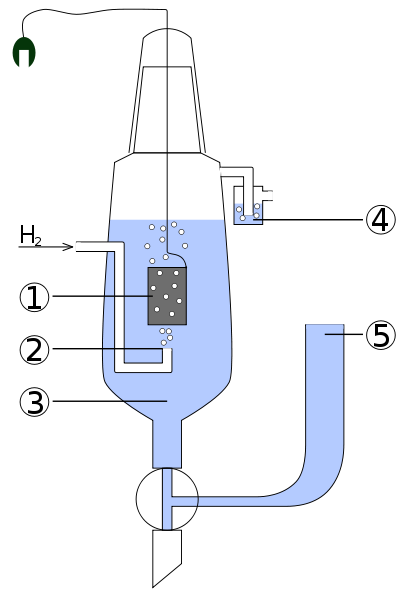
\includegraphics[width=\textwidth]{img/SVE.png}
			\caption*{Schéma SVE.\footnote[frame]{Zdroj: \href{https://commons.wikimedia.org/wiki/File:Standard_hydrogen_electrode_2009-02-06.svg}{Kaverin/Commons}}}
		\end{figure}
	\end{columns}
}

\section{Sloučeniny}
\subsection{Osmium}
\frame{
	\frametitle{}
	\vfill
	\begin{columns}
		\begin{column}{.5\textwidth}
		\begin{tabular}{|c|l|}
		\hline
		Ox. číslo & Sloučenina \\\hline
		$-$II & \ce{Na2[Os(CO)4]} \\\hline
		$-$I & \ce{Na2[Os4(CO)13]} \\\hline
		0 & \ce{[Os(CO)5], [Os3(CO)12]} \\\hline
		I & \ce{[Os(NH3)6]+} \\\hline
		II & \ce{OsI2} \\\hline
		III & \ce{OsBr3} \\\hline
		IV & \ce{OsO2}, \ce{OsCl4} \\\hline
		V & \ce{OsF5}, \ce{[OsCl6]-} \\\hline
		VI & \ce{[OsF6]}, \ce{[OsCl4N]-} \\\hline
		VII & \ce{OsOF5}, \ce{OsF7} \\\hline
		VIII & \ce{OsO4, K2[OsF2O4]} \\\hline
		\end{tabular}
		\end{column}
		\begin{column}{.5\textwidth}
			\begin{figure}
				\adjincludegraphics[width=\textwidth]{img/Triosmiumdodecacarbonyl.png}
			\end{figure}
		\end{column}
	\end{columns}
	\vfill
}

\frame{
	\frametitle{}
	\vfill
	\begin{columns}
		\begin{column}{.7\textwidth}
			\begin{itemize}
				\item Oxid osmičelý, \ce{OsO4}, je nažloutlá, těkavá  a silně toxická pevná látka.
				\item Nažloutlé zbarvení je způsobeno stopovými nečistotami \ce{OsO2}.
				\item Sublimuje za laboratorní teploty, je izoelektronový s manganistanem.
				\item Práškové osmium reaguje s kyslíkem za laboratorní teploty za vzniku \ce{OsO4}, v bulkovém stavu je nutné zahřívání až na 400~$^\circ$C.
				\item Je to Lewisova kyselina a mírné oxidační činidlo. Alkeny dokáže oxidovat na \textit{cis}-dioly.
			\end{itemize}
		\end{column}
		\begin{column}{.3\textwidth}
			\begin{figure}
				\adjincludegraphics[height=.4\textheight]{img/Osmiumtetroxide.jpg}
				\caption*{Oxid osmičelý.\footnote[frame]{Zdroj: \href{https://commons.wikimedia.org/wiki/File:Osmiumtetroxide1.jpg}{Vano3333/Commons}}}
			\end{figure}
		\end{column}
	\end{columns}

	\begin{figure}
		\adjincludegraphics[width=\textwidth]{img/Dihydroxylation_with_OsO4.png}
	\end{figure}
	\vfill
}

\frame{
	\frametitle{}
	\vfill
	\begin{columns}
		\begin{column}{.7\textwidth}
			\begin{itemize}
				\item S vodnými roztoky alkalických hydroxidů reaguje za vzniku komplexních aniontů \ce{[OsO4(OH)2]^{2-}}.
				\item Ty lze snadno redukovat na \ce{[OsO2(OH)4]^{2-}}.\footnote[frame]{\href{https://doi.org/10.1002/9780470132517.ch18}{Potassium Tetrahydroxodioxoosmate(VI) and trans-Bis(Ethylenediamine)Dioxoosmium(VI) Chloride}}
				\item \ce{2 OsO4 + C2H5OH + 5 KOH -> \\ CH3CO2K + 2 K2[OsO2(OH)4]}
				\item S aminy poskytuje imidové komplexy:
				\item \ce{OsO4 + ^tBuNH2 -> OsO3(N^tBu) + H2O}
				\item Reakcí s oxidem uhelnatým dochází k reduktivní karbonylaci. Vzniká triosmium dodekakarbonyl, \ce{Os3(CO)12}:\footnote[frame]{\href{https://doi.org/10.1021/ic50003a016}{The Molecular and Crystal Structure of \ce{Os3(CO)12}}}
				\item \ce{3 OsO4 + 24 CO -> Os3(CO)12 + 12 CO2}
			\end{itemize}
		\end{column}
		\begin{column}{.3\textwidth}
			\begin{figure}
				\adjincludegraphics[width=\textwidth]{img/CSD_CIF_KEWMEE.png}
				\caption*{Struktura \ce{^tBuNOsO3}.\footnote[frame]{Zdroj: \href{https://commons.wikimedia.org/wiki/File:CSD_CIF_KEWMEE.png}{Smokefoot/Commons}}}
			\end{figure}
		\end{column}
	\end{columns}
	\vfill
}

\frame{
	\frametitle{}
	\vfill
	\begin{figure}
		\adjincludegraphics[width=.85\textwidth]{img/Triosmiumdodecacarbonyl.png}
		\caption*{Struktura \ce{Os3(CO)12}.\footnote[frame]{Zdroj: \href{https://commons.wikimedia.org/wiki/File:Triosmiumdodecacarbonyl.svg}{Nothingserious/Commons}}}
	\end{figure}
	\vfill
}

\frame{
	\frametitle{}
	\vfill
	\textbf{Halogenidy a halogenid-oxidy osmia}
	\begin{center}
		\begin{tabular}{|c|c|c|c|c|}
			\hline
			VII & \ce{OsF7} & & & \\\hline
			VI & \ce{OsF6} & & & \\\hline
			V & \ce{OsF5} & \ce{OsCl5} & & \\\hline
			IV & \ce{OsF4} & \ce{OsCl4} & \ce{OsBr4} & \\\hline
			III &  & \ce{OsCl3} & \ce{OsBr3} & \ce{OsI3} \\\hline
			II &  & & & \ce{OsI2} \\\hline
			I & & & & OsI \\\hline
		\end{tabular}
	\end{center}
	\begin{itemize}
		\item Chemie halogenidů osmia je poměrně komplikovaná.\footnote[frame]{\href{https://doi.org/10.1021/ic0608290}{Osmium(VII) Fluorine Compounds}}
		\item Fluorid osmistý, \ce{OsF7}, byl připraven pouze jednou a to reakcí osmia s fluorem za vysoké teploty a tlaku. Pokud by se jeho existence prokázala, šlo by o třetí heptafluorid (\ce{IF7} a \ce{ReF7}).
		\item \ce{OsF6} získáme reakcí z prvků za zvýšené teploty:
		\item \ce{Os + 3 F2 ->[300 $^\circ$C] OsF6}
		\item Reakcí s \ce{OsO4} poskytuje řadu halogenid-oxidů.
	\end{itemize}
	\vfill
}

\frame{
	\frametitle{}
	\vfill
	\begin{figure}
		\adjincludegraphics[width=\textwidth]{img/OsO4-OsF6.png}
	\end{figure}
	\vfill
}

\frame{
	\frametitle{}
	\vfill
	\begin{itemize}
		\item \ce{OsO2F4} je fialová pevná látka s teplotou tání 90~$^\circ$C.
		\item Připravuje se fluorací \ce{OsO4} pomocí \ce{KrF2}:\footnote[frame]{\href{https://doi.org/10.1021/ja00077a029}{Osmium tetrafluoride dioxide, \ce{cis-OsO2F4}}}
		\item \ce{OsO4 + 2 KrF2 -> OsO2F4 + 2 Kr + O2}
		\item Stabilní je pouze izomer cis.
		\item Reakcí s \ce{AsF5} poskytuje kation \ce{[F(cis-OsO2F3)$^+_2$]}.
	\end{itemize}
	\begin{figure}
		\adjincludegraphics[width=\textwidth]{img/OsO2F4.png}
	\end{figure}
	\vfill
}

\frame{
	\frametitle{}
	\vfill
	\textbf{Sloučenina osmia v oxidačním stavu II}
	\begin{columns}
		\begin{column}{.7\textwidth}
		\begin{itemize}
		\item Halogenidy ani oxidy \ce{Os^{II}} nejsou příliš podrobně popsány.
		\item Zahříváním kovu se sírou vzniká disulfid \ce{OsS2}, který obsahuje anion \ce{S$^{2-}_2$}.
		\item Zahříváním kovového osmia a \ce{MgH2} v atmosféře vodíku vzniká komplexní hydrid \ce{Mg2[OsH6]}.
		\item Redukcí \ce{[OsCl6]^{2-}} pomocí \ce{N2H4} vzniká  komplex s \ce{N2} ligandem, ten lze dále redukovat dusitanem.
	\end{itemize}
	\end{column}
	\begin{column}{.3\textwidth}
	\begin{figure}
		\adjincludegraphics[width=\textwidth]{img/Os-NH3-N2.png}
	\end{figure}
	\end{column}
	\end{columns}
	\vfill
}

\frame{
	\frametitle{}
	\vfill
	\begin{columns}
		\begin{column}{.7\textwidth}
			\begin{itemize}
				\item \textbf{Osmocen} je bílá, pevná látka.
				\item Lze ji připravit refluxem \ce{OsO4} s kyselinou bromovodíkovou a následnou reakcí s kovovým zinkem a cyklopentadienem.\footnote[frame]{\href{https://doi.org/10.1007/BF01161040}{Crystal structure of osmocene, \ce{Os(\eta-C5H5)2}}}
				\item Cyklopentadienidové ligandy jsou, na rozdíl od ferrocenu, v zákrytové konformaci.
				\item Poměrně ochotně vytváří adukty s Lewisovskými kyselinami.
				\item Kation \ce{[Os(C5H5)2]+} vytváří dimer obsahující vazbu \ce{Os-Os}.\footnote[frame]{\href{https://doi.org/10.1021/ic00255a023}{Higher oxidation state chemistry of osmocene: dimeric nature of the osmocenium ion}}
			\end{itemize}
		\end{column}
		\begin{column}{.3\textwidth}
			\begin{figure}
				\adjincludegraphics[width=\textwidth]{img/Osmocene.png}
				\caption*{Osmocen.\footnote[frame]{\href{https://en.wikipedia.org/wiki/File:Osmocene_Eclipsed_Conformer_Structural_Formula.svg}{Zdroj: Bert.Kilanowski/Commons}}}
			\end{figure}
		\end{column}
	\end{columns}
	\vfill
}

\frame{
	\frametitle{}
	\vfill
	\begin{figure}
		\adjincludegraphics[height=.8\textwidth,rotate=90]{img/FERXUV.png}
		\caption*{Struktura dimeru \ce{[(OsCp2)2][PF6]2}\footnote[frame]{\href{https://doi.org/10.1021/ic00255a023}{Higher oxidation state chemistry of osmocene: dimeric nature of the osmocenium ion}}}
	\end{figure}
	\vfill
}

\subsection{Iridium}
\frame{
	\frametitle{}
	\vfill
	\begin{columns}
		\begin{column}{.5\textwidth}
			\begin{tabular}{|c|l|}
				\hline
				Ox. číslo & Sloučenina \\\hline
				$-$III & \ce{[Ir(CO)3]^{3-}} \\\hline
				$-$I & \ce{[Ir(CO)3(PPh3)]-} \\\hline
				0 & \ce{[Ir4(CO)12]} \\\hline
				I & \ce{[Ir(CO)Cl(PPh3)2]} \\\hline
				II & \ce{IrCl2} \\\hline
				\textbf{III} & \textbf{\ce{IrCl3}} \\\hline
				IV & \ce{IrO2} \\\hline
				V & \ce{Ir4F20} \\\hline
				VI & \ce{[IrF6]}\\\hline
				VII & \ce{[($\eta$^2-O2)IrO2]+} \\\hline
				VIII & \ce{IrO4} \\\hline
				IX\footnote[frame]{\href{https://doi.org/10.1038/nature13795}{Identification of an iridium-containing compound with a formal oxidation state of IX}} & \ce{[IrO4]+} \\\hline
			\end{tabular}
		\end{column}
		\begin{column}{.5\textwidth}
			\begin{figure}
				\adjincludegraphics[width=\textwidth]{img/Ir4CO12.png}
				\caption*{Dodekakarbonyl tetrairidia, \ce{Ir4(CO)12}.\footnote[frame]{\href{https://commons.wikimedia.org/wiki/File:Ir4(CO)12.svg}{Zdroj: Smokefoot/Commons}}}
			\end{figure}
		\end{column}
	\end{columns}
	\vfill
}

\frame{
	\frametitle{}
	\vfill
	\textbf{Halogenidy iridia} \\
	\begin{tabular}{|c|c|c|c|c|}
		\hline
		Ox. č. & Fluoridy & Chloridy & Bromidy & Jodidy \\\hline
		VI & \ce{IrF6} (žlutý) & & & \\\hline
		V & \ce{[IrF5]4} (žlutý) & & & \\\hline
		IV & \ce{IrF4} (červený) & & & \\\hline
		III & \ce{IrF3} (černý) & \ce{IrCl3} (červený) & \ce{IrBr3} (červ.hnědý) & \ce{IrI3} (hnědý) \\\hline
	\end{tabular}

	\begin{figure}
		\adjincludegraphics[height=.4\textheight]{img/Ir4F20.png}
	\end{figure}
	\vfill
}

\frame{
	\frametitle{}
	\vfill
	\textbf{Halogenidy iridia} \\
	\begin{itemize}
		\item \ce{IrF6} je výchozí látkou pro přípravu jediného známého karbonylového komplexu s kovem v oxidačním stavu III:\footnote[frame]{\href{https://doi.org/10.1002/anie.199619741}{Cationic Iridium(III) Carbonyl Complexes}}
		\item \ce{2 IrF6 + 12 SbF5 + 15 CO -> 2 [Ir(CO)6][Sb2F11]3 + 3 COF2}
		\item \ce{IrF5} vzniká přímou reakcí prvků, má tetramerní strukturu analogickou s \ce{NbF5}.
		\item \ce{2 Ir + 5 F2 ->[400 $^\circ$C] 2 IrF5}
		\item S vodou reaguje za uvolňování kyslíku:
		\item \ce{4 IrF5 + 10 H2O -> 4 IrO2 + 20 HF + O2}
		\item V roztoku HF nebo \ce{IF5} poskytují komplexní anionty:
		\item \ce{IrF5 + KF ->[HF, IF5] K[IrF6]}
	\end{itemize}
	\vfill
}

\frame{
	\frametitle{}
	\vfill
	\textbf{Halogenidy iridia} \\
	\begin{itemize}
		\item V oxidačním stavu IV známe pouze fluorid, chlorid nebyl dosud připraven, ale známe soli hexachloridoiridičité, které jsou důležité výchozí látky v chemii iridia:
	\end{itemize}

	\begin{figure}
		\adjincludegraphics[width=\textwidth]{img/IrCl6-2-.png}
	\end{figure}
	\vfill
}

\frame{
	\frametitle{}
	\vfill
	\textbf{Halogenidy iridia} \\
	\begin{itemize}
		\item \textbf{Fluorid iriditý}, \ce{IrF3}, můžeme připravit redukcí \ce{IrF6} kovovým iridiem:
		\item \ce{IrF6 + Ir ->[500 $^\circ$C] 2 IrF3}
		\item \textbf{Chlorid iriditý}, \ce{IrCl3}, se běžně vyskytuje jako trihydrát.
		\item Bezvodý $\alpha$-\ce{IrCl3} má vrstevnatou strukturu izomorfní s \ce{AlCl3}.
		\item Zahříváním hnědé $\alpha$ modifikace na teplotu 600–800~°C dojde k přechodu na červenou, romboedrickou modifikaci $\beta$.\footnote[frame]{\href{https://doi.org/10.1002/zaac.19653390109}{Die Kristallstruktur von $\beta$-Iridium(III)-Chlorid}}
		\item Trihydrát (\ce{IrCl3.3H2O}) má tmavě zelenou barvu. Je komerčně dostupný a slouží jako výchozí sloučenina pro syntézu jiných sloučenin iridia:
		\item \ce{IrCl3.3H2O + 3 CH3CN ->[reflux] [IrCl3(NCCH3)3] + 3 H2O}
		\item \ce{IrCl3.3H2O + 2 bpy -> cis-[IrCl2(bpy)2]Cl + 3 H2O}
	\end{itemize}
	\vfill
}

\frame{
	\frametitle{}
	\vfill
	\begin{columns}
		\begin{column}{.5\textwidth}
			\begin{figure}
				\adjincludegraphics[width=\textwidth]{img/Alpha-IrCl3.png}
				\caption*{Krystalová struktura $\alpha$-\ce{IrCl3}.\footnote[frame]{\href{https://commons.wikimedia.org/wiki/File:Alpha-iridium(III)-chloride-xtal-viewed-down-b-axis-3D-bs-17.png}{Zdroj: Ben Mills/Commons}}}
			\end{figure}
		\end{column}

		\begin{column}{.5\textwidth}
			\begin{figure}
				\adjincludegraphics[width=1.1\textwidth]{img/Beta-IrCl3.png}
				\caption*{Krystalová struktura $\beta$-\ce{IrCl3}.\footnote[frame]{\href{https://commons.wikimedia.org/wiki/File:Beta-iridium(III)-chloride-xtal-viewed-down-ab-diagonal-3D-bs-17-raw.png}{Zdroj: Ben Mills/Commons}}}
			\end{figure}
		\end{column}
	\end{columns}
	\vfill
}

\frame{
	\frametitle{}
	\vfill
	\begin{itemize}
		\item Jediným potvrzeným oxidem iridia je \ce{IrO2}, krystaluje ve struktuře rutilu.
		\item Krystalová struktura obsahuje oktaedricky koordinované ionty iridia a planárně trigonální oxidové anionty.
		\item Je to černá, pevná látka stabilní do teploty 1100~$^\circ$C.
		\item Připravuje se oxidací chloridu iriditého:
		\item \ce{2 IrCl3 + 2 O2 -> 2 IrO2 + 3 Cl2}
		\item Fotochemickou reakcí s kyslíkem v argonové matrici při teplotě 6~K dochází k~přesmyku peroxokomplexu za vzniku nestabilního \ce{IrO4}.\footnote[frame]{\href{https://doi.org/10.1002/ange.200902733}{Formation and Characterization of the Iridium Tetroxide Molecule with Iridium in the Oxidation State +VIII}}
	\end{itemize}

	\begin{figure}
		\adjincludegraphics[width=.65\textwidth]{img/IrO4.png}
	\end{figure}
	\vfill
}

\frame{
	\frametitle{}
	\vfill
	\begin{itemize}
		\item \textbf{Tris(2-fenylpyridin)iriditý komplex}, \ce{ [Ir(ppy)3]}, žlutozelená pevná látka.\footnote[frame]{\href{https://doi.org/10.1021/ic00008a003}{A new synthetic route to the preparation of a series of strong photoreducing agents: fac-tris-ortho-metalated complexes of iridium(III) with substituted 2-phenylpyridines}}
		\item Tento komplex je studován jako fotoredoxní katalyzátor.
		\item Vykazuje elektroluminiscenci\footnote{Luminiscence vyvolaná průchodem elektrického proudu}, emituje zelené záření.
		\item Připravuje se z acetylacetonátu iriditého.
	\end{itemize}

	\begin{figure}
		\adjincludegraphics[width=.8\textwidth]{img/Ir-ppy.png}
	\end{figure}
	\vfill
}

\frame{
	\frametitle{}
	\vfill
	\begin{columns}
		\begin{column}{.5\textwidth}
			\begin{itemize}
				\item \textbf{Dodekakarbonyl tetrairidia}, \ce{Ir4(CO)12}, je sloučenina iridia v oxidačním stavu 0.
				\item Je stabilní na vzduchu a velmi špatně rozpustný v organických rozpouštědlech.
				\item Molekula má tetraedrickou symetrii (T$_d$), atomy iridia jsou koordinovány oktaedricky.\footnote[frame]{\href{https://doi.org/10.1021/ic50190a040}{Crystal structure of tetrairidium dodecacarbonyl, \ce{Ir4(CO)12}. An unpleasant case of disorder}}
				\item Připravuje se redukcí chloridu iriditého:
			\end{itemize}
		\end{column}

		\begin{column}{.4\textwidth}
			\begin{figure}
				\adjincludegraphics[width=1\textwidth]{img/Ir4CO12.png}
				\caption*{Struktura \ce{Ir4(CO)12}.\footnote[frame]{\href{https://en.wikipedia.org/wiki/File:Ir4(CO)12.svg}{Zdroj: Smokefoot/Commons}}}
			\end{figure}
		\end{column}
	\end{columns}
	\begin{align*}
		\ce{IrCl3 + 3 CO + H2O &-> [Ir(CO)2Cl2]- + CO2 + 2 H+ + Cl-}\\
		\ce{4 [Ir(CO)2Cl2]- + 6 CO + 2 H2O &-> Ir4(CO)12 + 2 CO2 + 4 H+ + 8 Cl-}
	\end{align*}
	\vfill
}

\subsection{Platina}
\frame{
	\frametitle{}
	\vfill
			\begin{center}
				\begin{tabular}{|c|l|}
					\hline
					Ox. číslo & Sloučenina \\\hline
					0 & \ce{[Pt(PF3)4]} \\\hline
					II & \ce{PtCl$_4^{2-}$} \\\hline
					IV & \ce{PtCl$_6^{2-}$}; \ce{Pt($\eta$^5-C5H5)Me3} \\\hline
					V & \ce{[PtF6]-} \\\hline
					VI & \ce{[PtF6]}\\\hline
				\end{tabular}
			\end{center}
			\begin{figure}
				\adjincludegraphics[width=.4\textwidth]{img/Cl2Ptcod.png}
			\end{figure}
	\vfill
}

\frame{
	\frametitle{}
	\vfill
		\begin{itemize}
			\item Komplexy iontů s konfigurací d$^8$ (\ce{Rh^I}, \ce{Ir^I}, \ce{Pd^{II}}, \ce{Pt^{II}} a \ce{Au^{III}}) preferují čtvercovou geometrii oproti tetraedrické.
			\item Tomu odpovídá i jiná struktura štěpení d-orbitalů.\footnote[frame]{\href{https://chem.libretexts.org/Bookshelves/Inorganic_Chemistry/Supplemental_Modules_and_Websites_(Inorganic_Chemistry)/Crystal_Field_Theory/Crystal_Field_Theory}{Crystal Field Theory}}
			\item Protože v ose \textit{z} nejsou žádné ligandy, dojde ke snížení energie příslušných d-orbitalů.
			\item Čtvercové komplexy jsou zpravidla nízkospinové.
			\item Příkladem je cisplatina, \ce{[PtCl2(NH3)2]}.
		\end{itemize}
		\begin{figure}
			\adjincludegraphics[height=.33\textheight]{img/Square_planar_splitting_diagram.png}
			\caption*{Štěpení MO ve čtvercovém komplexu.\footnote[frame]{Zdroj: \href{https://commons.wikimedia.org/wiki/File:Square_planar_splitting_diagram.svg}{YanA/Commons}}}
		\end{figure}
	\vfill
}

\frame{
	\frametitle{}
	\vfill
	\begin{itemize}
		\item \textit{Cisplatina}, \ce{[PtCl2(NH3)2]}, léčivo používané k léčbě mnoha druhů rakoviny. Aplikuje se injekčně.\footnote[frame]{\href{https://zdravi.euro.cz/clanek/postgradualni-medicina/molekularni-mechanismy-ucinku-cisplatiny-455575}{Molekulární mechanismy účinku cisplatiny}}
		\item Poprvé byla připravena v roce 1845, k léčbě se používá od roku 1978.\footnote[frame]{\href{https://doi.org/10.1021/acscentsci.3c01340}{Metals in Cancer Research: Beyond Platinum Metallodrugs}}
		\item Její strukturu určil Alfred Werner v roce 1893.\footnote[frame]{\href{https://doi.org/10.1021/cen-v083n025.p052}{Cisplatin}}
		\item V současnosti se studuje velká množina derivátů cisplatiny.
		\item Připravuje se z tetrachloroplatičitanu.
		\item \ce{Pt ->[HCl + HNO3, KCl] K2PtCl6 ->[SO2] K2PtCl4}
	\end{itemize}
	\begin{figure}
		\adjincludegraphics[height=.2\textheight]{img/Cisplatin-stereo.png}
	\end{figure}
	\vfill
}

\frame{
	\frametitle{}
	\vfill
	\begin{figure}
		\adjincludegraphics[width=1.05\textwidth]{img/Cisplatin_synthesis.png}
		\caption*{Syntéza cisplatiny.\footnote[frame]{Zdroj: \href{https://commons.wikimedia.org/wiki/File:Cisplatin_synthesis.svg}{Anypodetos/Commons}}}
	\end{figure}
	\vfill
}

\frame{
	\frametitle{}
	\vfill
	\begin{itemize}
		\item \textit{Karboplatina}, paraplatina, je další léčivo používané k léčbě  rakoviny založené na platině.
		\item Patentována byla v roce 1972, v medicíně se používá od roku 1986.
		\item Připravuje se reakcí cisplatiny s dusičnanem stříbrným a poté s kyselinou cyklobutan-1,1-dikarboxylovou.
	\end{itemize}
	\begin{columns}
		\begin{column}{.5\textwidth}
			\begin{figure}
				\adjincludegraphics[height=.35\textheight]{img/Carboplatin-skeletal.png}
				\caption*{Karboplatina.\footnote[frame]{Zdroj: \href{https://commons.wikimedia.org/wiki/File:Carboplatin-skeletal.svg}{Catclock/Commons}}}
			\end{figure}
		\end{column}

		\begin{column}{.5\textwidth}
			\begin{figure}
				\adjincludegraphics[height=.35\textheight]{img/Carboplatin.png}
				\caption*{Kuličkový model karboplatiny.\footnote[frame]{Zdroj: \href{https://commons.wikimedia.org/wiki/File:Carboplatin-from-xtal-view-1-Mercury-3D-balls.png}{Ben Mills/Commons}}}
			\end{figure}
		\end{column}
	\end{columns}
	\vfill
}

\frame{
	\frametitle{}
	\vfill
	\begin{figure}
		\adjincludegraphics[height=.8\textheight]{img/Pt-leciva.png}
	\end{figure}
	\vfill
}

\frame{
	\frametitle{}
	\vfill
	\begin{itemize}
		\item \textit{Trans efekt} je jev, pozorovaný nejčastěji u čtvercových komplexů, kdy určité ligandy usnadňují substituci v poloze \textit{trans}.
		\item Tento jev byl studován především u platnatých komplexů.
		\item Trans efekt vysvětluje řada teorií, nejpravděpodobnějším důvodem je odčerpávání $\pi$ elektronů z atomu kovu. Proto jsou nejsilnější $\pi$-akceptorní ligandy.
	\end{itemize}

	\begin{center}
		\ce{F-}, \ce{H2O} $<$ \ce{NH3} $<$ \ce{py} $<$ \ce{Cl-} $<$ \ce{Br-} $<$ \ce{I-} $<$ \ce{H-} $<$ CO, \ce{CN-}
	\end{center}
	\vfill
}

\frame{
	\frametitle{}
	\vfill
	\begin{figure}
		\adjincludegraphics[width=\textwidth]{img/Synthesis_Cisplatin.png}
		\caption*{Syntéza cisplatiny.\footnote[frame]{Zdroj: \href{https://commons.wikimedia.org/wiki/File:Synthesis_Cisplatin_(trans_effect).svg}{Sponk/Commons}}}
	\end{figure}
	\begin{figure}
		\adjincludegraphics[width=\textwidth]{img/Synthesis_Transplatin.png}
		\caption*{Syntéza transplatiny.\footnote[frame]{Zdroj: \href{https://commons.wikimedia.org/wiki/File:Synthesis_Transplatin_(trans_effect).svg}{Sponk/Commons}}}
	\end{figure}
	\begin{center}
		\ce{F-}, \ce{H2O} $<$ \ce{NH3} $<$ \ce{py} $<$ \ce{Cl-} $<$ \ce{Br-} $<$ \ce{I-} $<$ \ce{H-} $<$ CO, \ce{CN-}
	\end{center}
	\vfill
}

\frame{
	\frametitle{}
	\vfill
	\begin{itemize}
		\item \textit{Magnusova zelená sůl} je sloučenina pojmenovaná po německém chemikovi Heinrichu Gustavovi Magnusovi, který ji objevil.
		\item Jde o tetrachloroplatnatan tetraamminplatnatý, \ce{[Pt(NH3)4][PtCl4]}.
		\item Je to nerozpustná polymerní sloučenina.\footnote[frame]{\href{https://doi.org/10.1002/9780470132333.ch80}{Tetrammineplatinum(II) Chloride: (Tetrammineplatinous Chloride)}}
		\item Známe i její polymorf, který má růžovou barvu.\footnote[frame]{\href{https://doi.org/10.1021/ja4076277}{Unravelling the Structure of Magnus’ Pink Salt}}
	\end{itemize}

	\begin{figure}
		\adjincludegraphics[width=.5\textwidth]{img/Magnus-green-salt.png}
		\caption*{Krystalová struktura Magnusovy zelené soli.\footnote[frame]{\href{https://commons.wikimedia.org/wiki/File:Magnus\%27-green-salt-from-xtal-1957-CM-3D-balls-horizontal.png}{Zdroj: Ben Mills/Commons}}}
	\end{figure}
	\vfill
}

\frame{
	\frametitle{}
	\vfill
	\begin{itemize}
		\item \ce{O2PtF6} je první připravenou sloučeninou obsahující dioxygenylový kation, \ce{O$_2^+$}.\footnote[frame]{\href{https://doi.org/10.1039/JR9620005253}{1005. Fluorides of the noble metals. Part II. Dioxygenyl hexafluoroplatinate(V), \ce{O2+[PtF6]-}}}
		\item Poprvé byla připravena reakcí platiny se směsí fluoru a kyslíku.
		\item \ce{Pt + O2 + 3 F2 ->[450 $^\circ$C] O2PtF6}
		\item Za nižší teploty vzniká pouze \ce{PtF4}
		\item Lze ho připravit i reakcí \ce{PtF6} s kyslíkem.
		\item Řád vazby v kationtu \ce{O$_2^+$} je 2,5, délka vazby 112,3~pm.
		\item Je paramagnetický.
	\end{itemize}
	\vfill
}

\frame{
	\frametitle{}
	\vfill
	\begin{itemize}
		\item Pro chemii platiny a dalších platinových kovů je důležitá \textit{lučavka královská}.
		\item Jde o směs koncentrované kyseliny chlorovodíkové a dusičné v poměru 3:1.
		\item Po jejich smísení dojde ke vzniku nitrosylchloridu a chloru:
		\item \ce{HNO3 + 3 HCl -> NOCl + Cl2 + 2 H2O}
	\end{itemize}

	\begin{figure}
		\adjincludegraphics[height=.42\textheight]{img/Aqua_regia.jpg}
		\caption*{Lučavka královská.\footnote[frame]{Zdroj: \href{https://commons.wikimedia.org/wiki/File:Aqua_regia_in_Davenport_Laboratories.jpg}{Thejohnnler/Commons}}}
	\end{figure}
	\vfill
}

\frame{
	\frametitle{}
	\vfill
	\begin{itemize}
		\item Rozpouštění kovové platiny probíhá za vzniku \ce{NO2} nebo NO a oxidace platiny na kyselinu platiničitou, \ce{H2PtCl6}.
		\item \ce{Pt + 4 NO$_3^-$ + 8 H+ -> Pt$^{4+}$ + 4 NO2 + 4 H2O}
		\item \ce{3 Pt + 4 NO$_3^-$ + 16 H+ -> 3 Pt$^{4+}$ + 4 NO + 8 H2O}
	\end{itemize}
	\vfill
	\begin{itemize}
		\item Následně dojde k reakci s chloridovými ionty:
		\item \ce{Pt$^{4+}$ + 6 Cl- -> PtCl$_6^{2-}$}
	\end{itemize}
	\vfill
	\begin{itemize}
		\item Průběh reakce je ve skutečnosti složitější, dochází i ke vzniku nitrosylových solí:
		\item \ce{2 Pt + 2 HNO3 + 8 HCl -> (NO)2PtCl4 + H2PtCl4 + 4 H2O}
		\item \ce{(NO)2PtCl4 + 2 HCl -> H2PtCl4 + 2 NOCl}
		\item \ce{H2PtCl4 + Cl2 -> H2PtCl6}
	\end{itemize}
	\vfill
}

\frame{
	\frametitle{}
	\vfill
	\begin{itemize}
		\item \ce{Pt ->[lucavka, KCl] K2PtCl6}
		\item \ce{K2PtCl6 ->[BrF3] K2PtF6}
		\item \ce{Pd ->[lucavka, KCl] K2PdCl6}
	\end{itemize}
	\begin{columns}
		\begin{column}{.33\textwidth}
			\begin{figure}
				\adjincludegraphics[height=.25\textheight]{img/Plaatina_reageerimine_kuningveega_01.jpg}
			\end{figure}
		\end{column}

		\begin{column}{.33\textwidth}
			\begin{figure}
				\adjincludegraphics[height=.25\textheight]{img/Plaatina_reageerimine_kuningveega_02.jpg}
			\end{figure}
		\end{column}

		\begin{column}{.33\textwidth}
			\begin{figure}
				\adjincludegraphics[height=.25\textheight]{img/Plaatina_reageerimine_kuningveega_03.jpg}
			\end{figure}
		\end{column}
	\end{columns}

	Průběh rozpouštění platiny v lučavce královské\footnote[frame]{\href{https://www.youtube.com/watch?v=APxL87X92t4}{Platinum Bar Dissolving in Acid (Aqua Regia)}}
	\vfill
}

\input{../Last}

\end{document}